\section{Benchmarking}
\label{sec:res_bench}
This section presents the result from the IOZone benchmarking tests run on each filesystem. The output result is divided into a table for each test for each filesystem. Each table presents the benchmark performance of the test for each file size and each buffer size. It is a table of five rows and 13 columns, where each cell is the performance of the test with the specific file size and buffer size. The complete data tables and graphs presenting the performance of each file system for the different file sizes can be found in Appendix~\ref{app:bench_data}.

Combining all the data in one table, we get the overall performance of a test. Using this data, we can plot a box plot presenting the spread of the values in the table. Figure~\ref{fig:res_box_ffs} presents a box plot of the benchmarking results of FFS, Figure~\ref{fig:res_box_fffs} presents a box plot of the benchmarking results of FFFS, and Figure~\ref{fig:res_box_apfs} presents a box plot of the benchmarking results of APFS. 

\begin{figure}[!htb]
	\label{fig:res_box_ffs}
	\begin{center}
		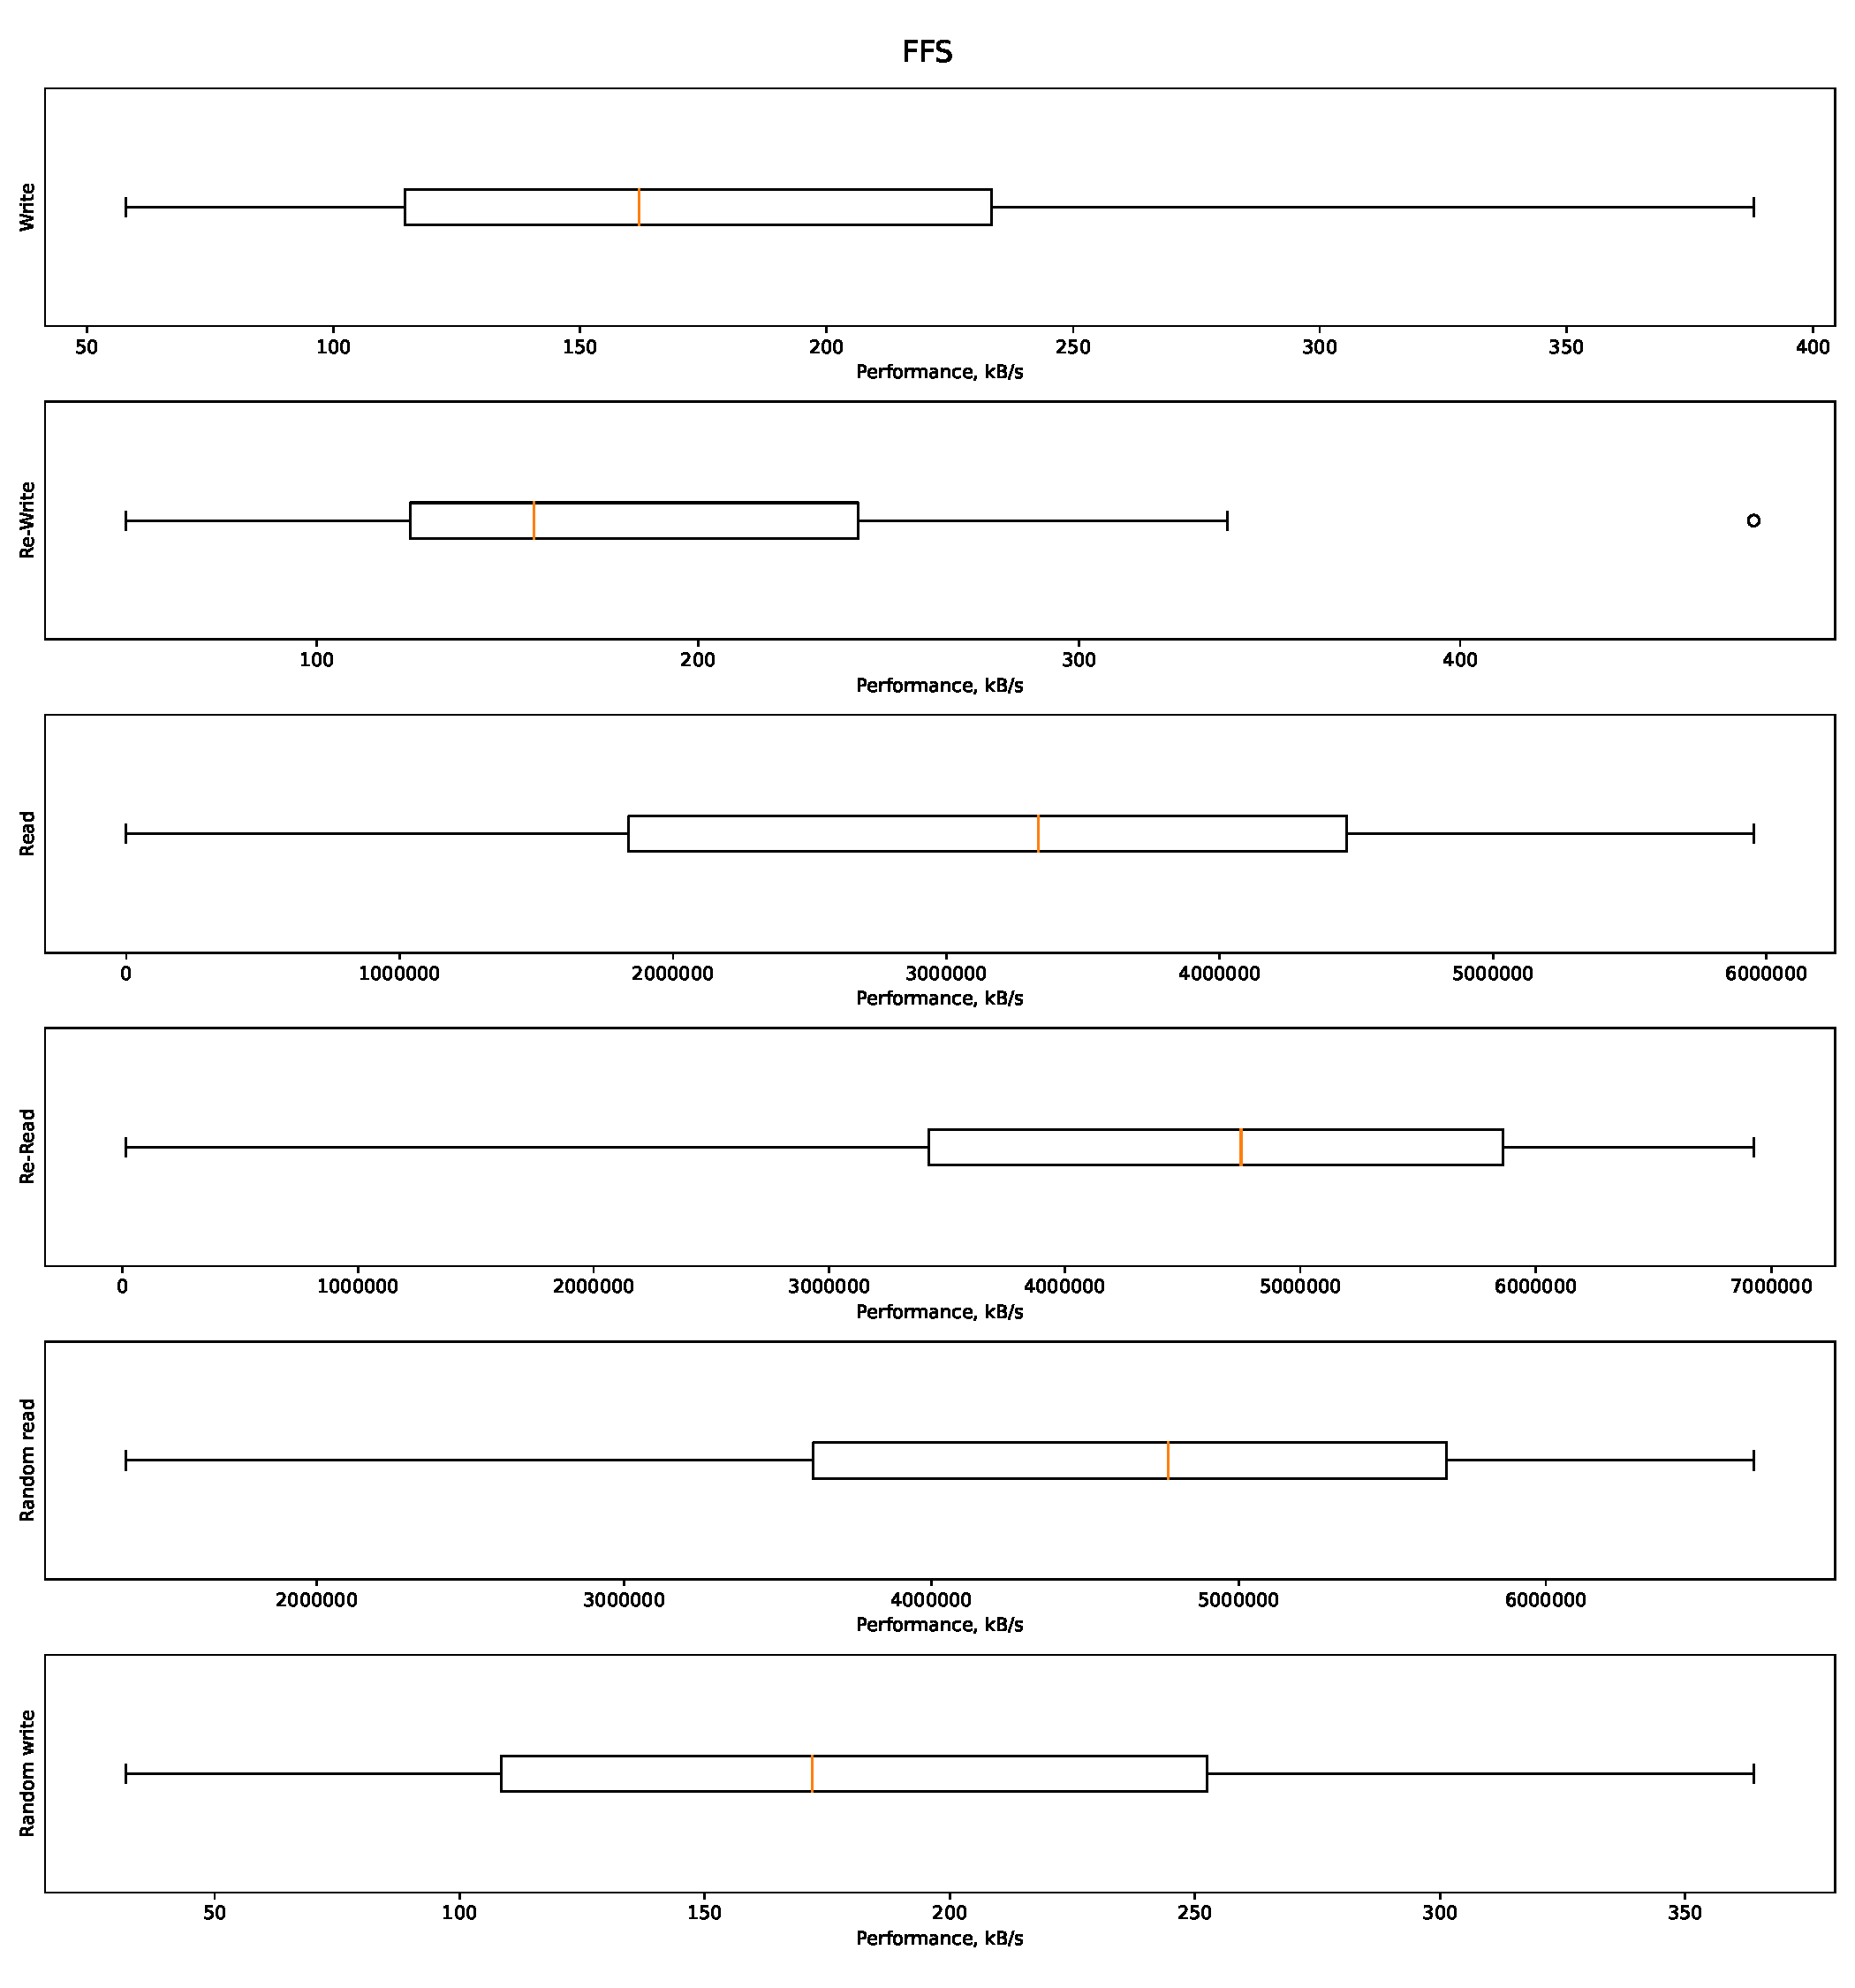
\includegraphics[width=1.0\textwidth]{figures/benchmarking/ffs/FFS-box.pdf}
	\end{center}
	\caption{Box plot of the IOZone output for the different tests for FFS}
\end{figure}

\begin{figure}[!htb]
	\label{fig:res_box_fffs}
	\begin{center}
		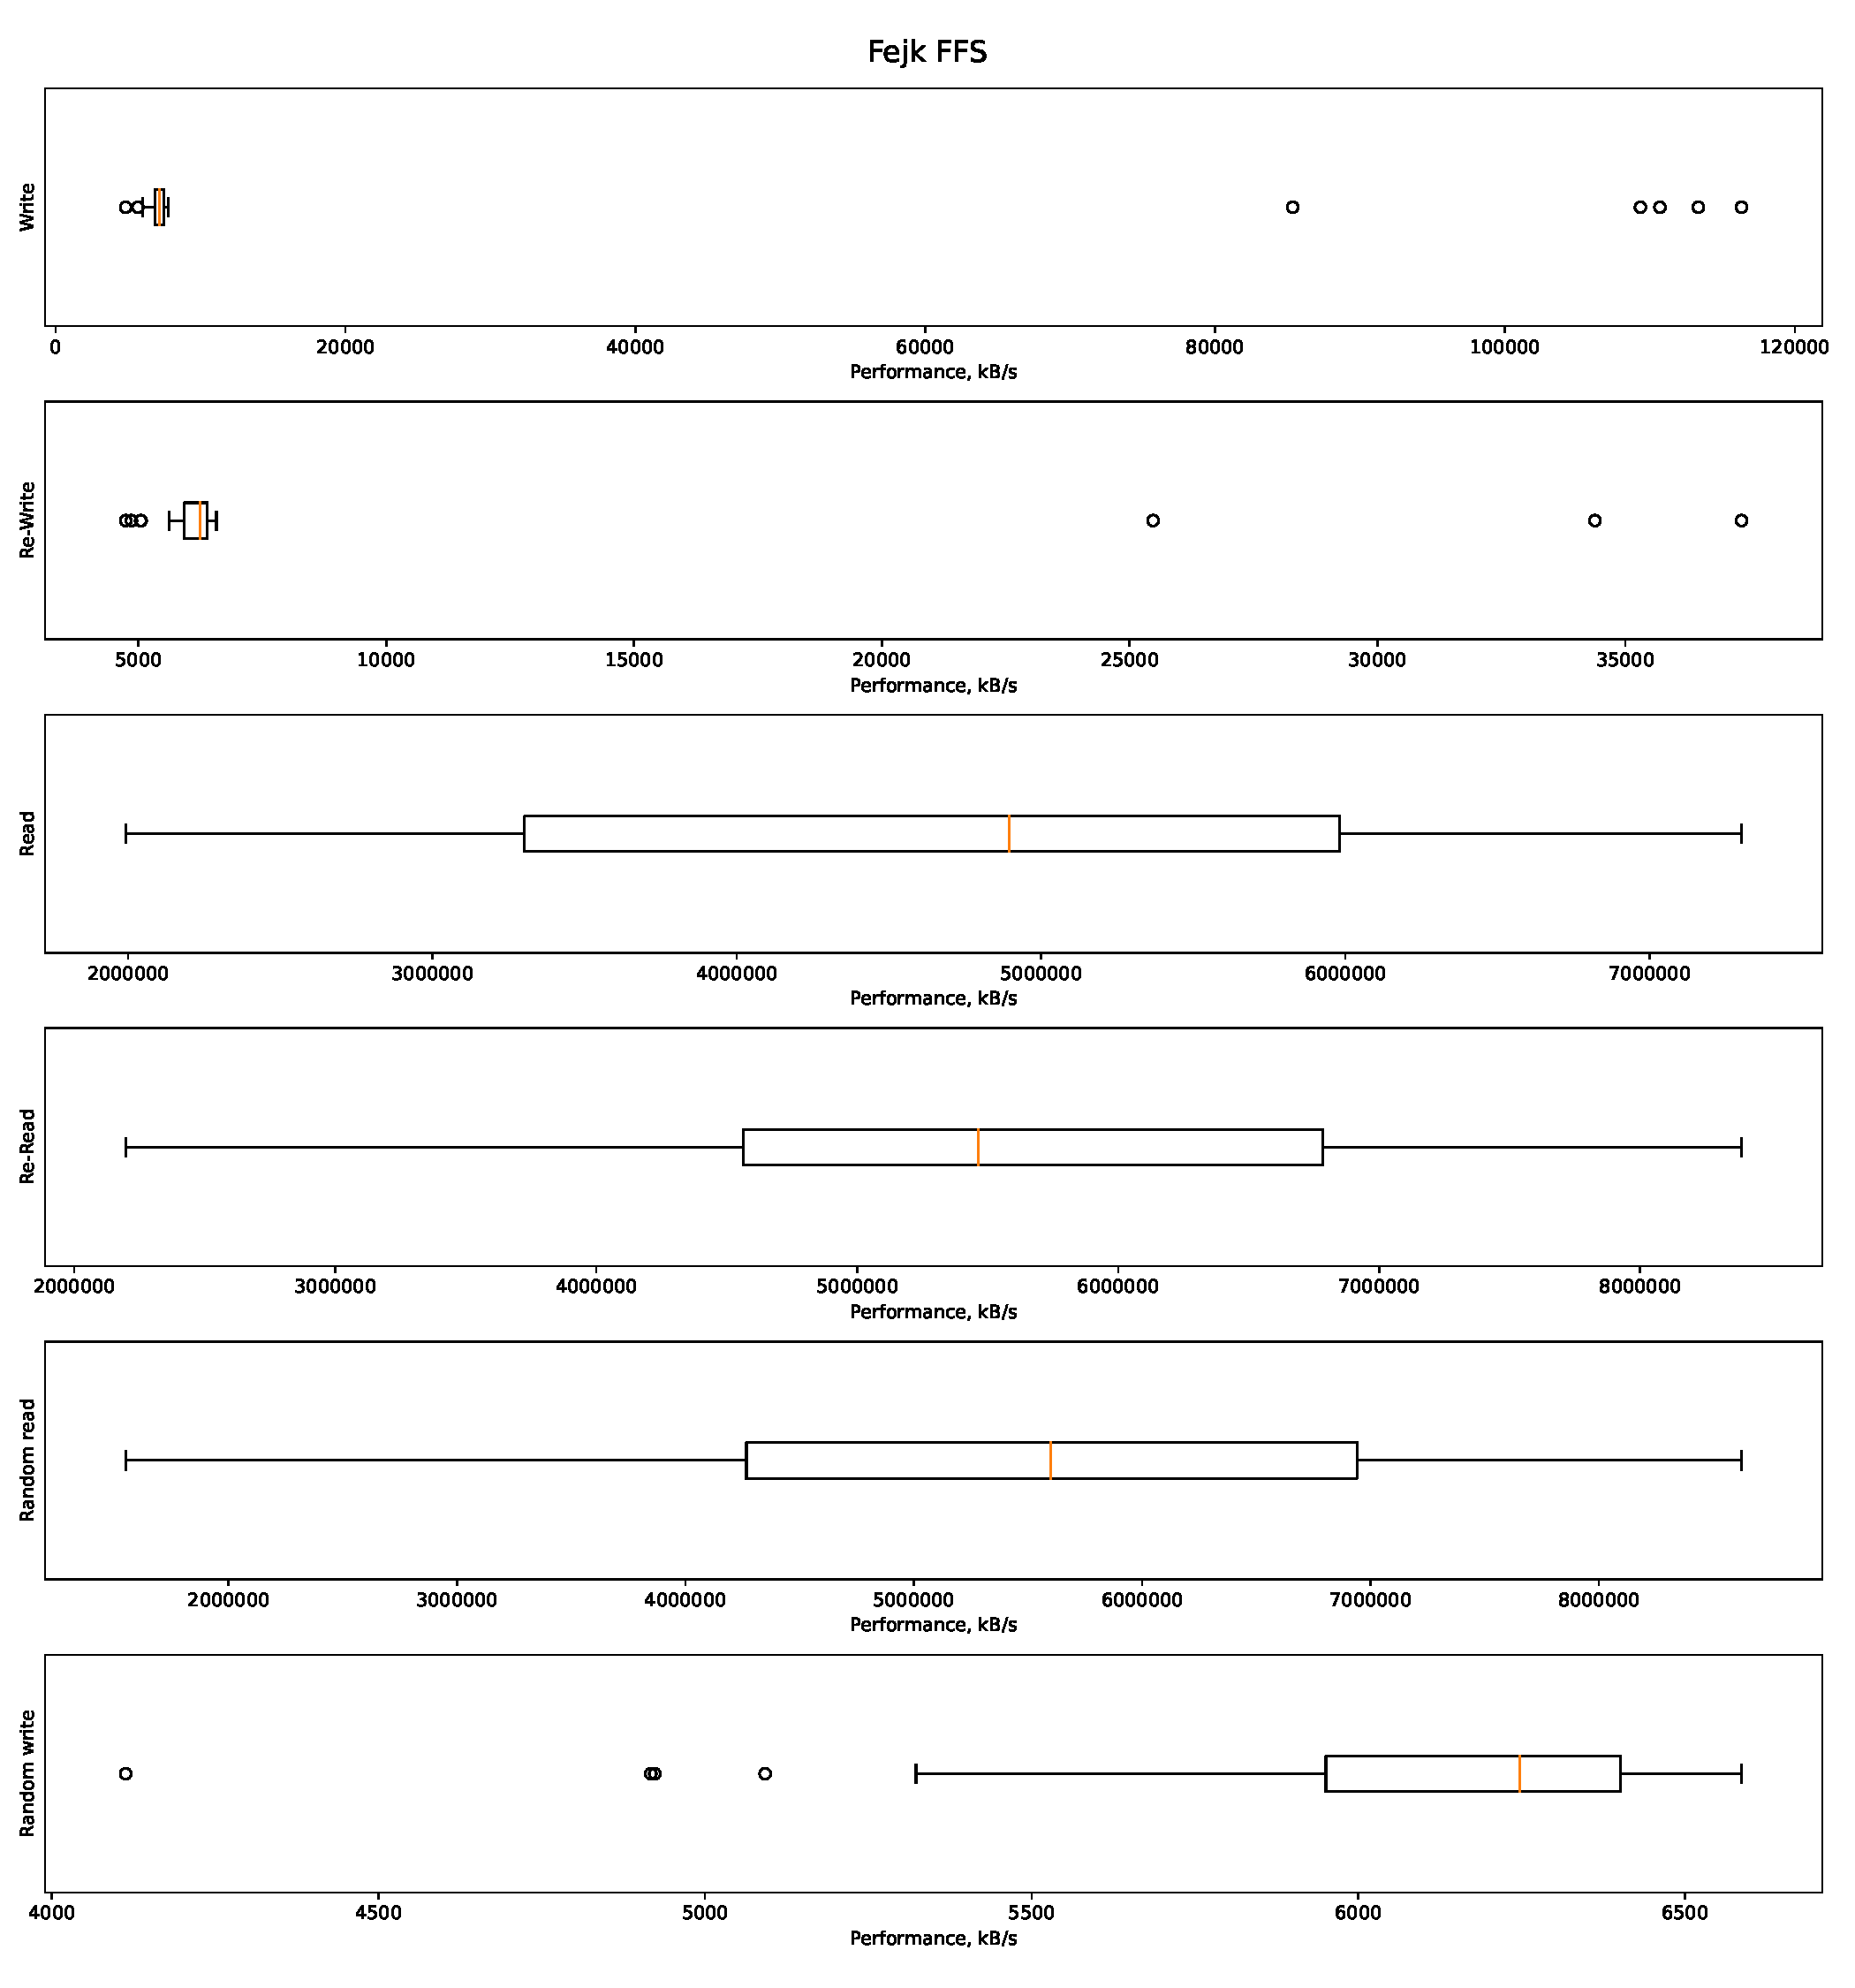
\includegraphics[width=1.0\textwidth]{figures/benchmarking/fake-ffs/Fejk FFS-box.pdf}
	\end{center}
	\caption{Box plot of the IOZone output for the different tests for FFFS}
\end{figure}

\begin{figure}[!htb]
	\label{fig:res_box_apfs}
	\begin{center}
		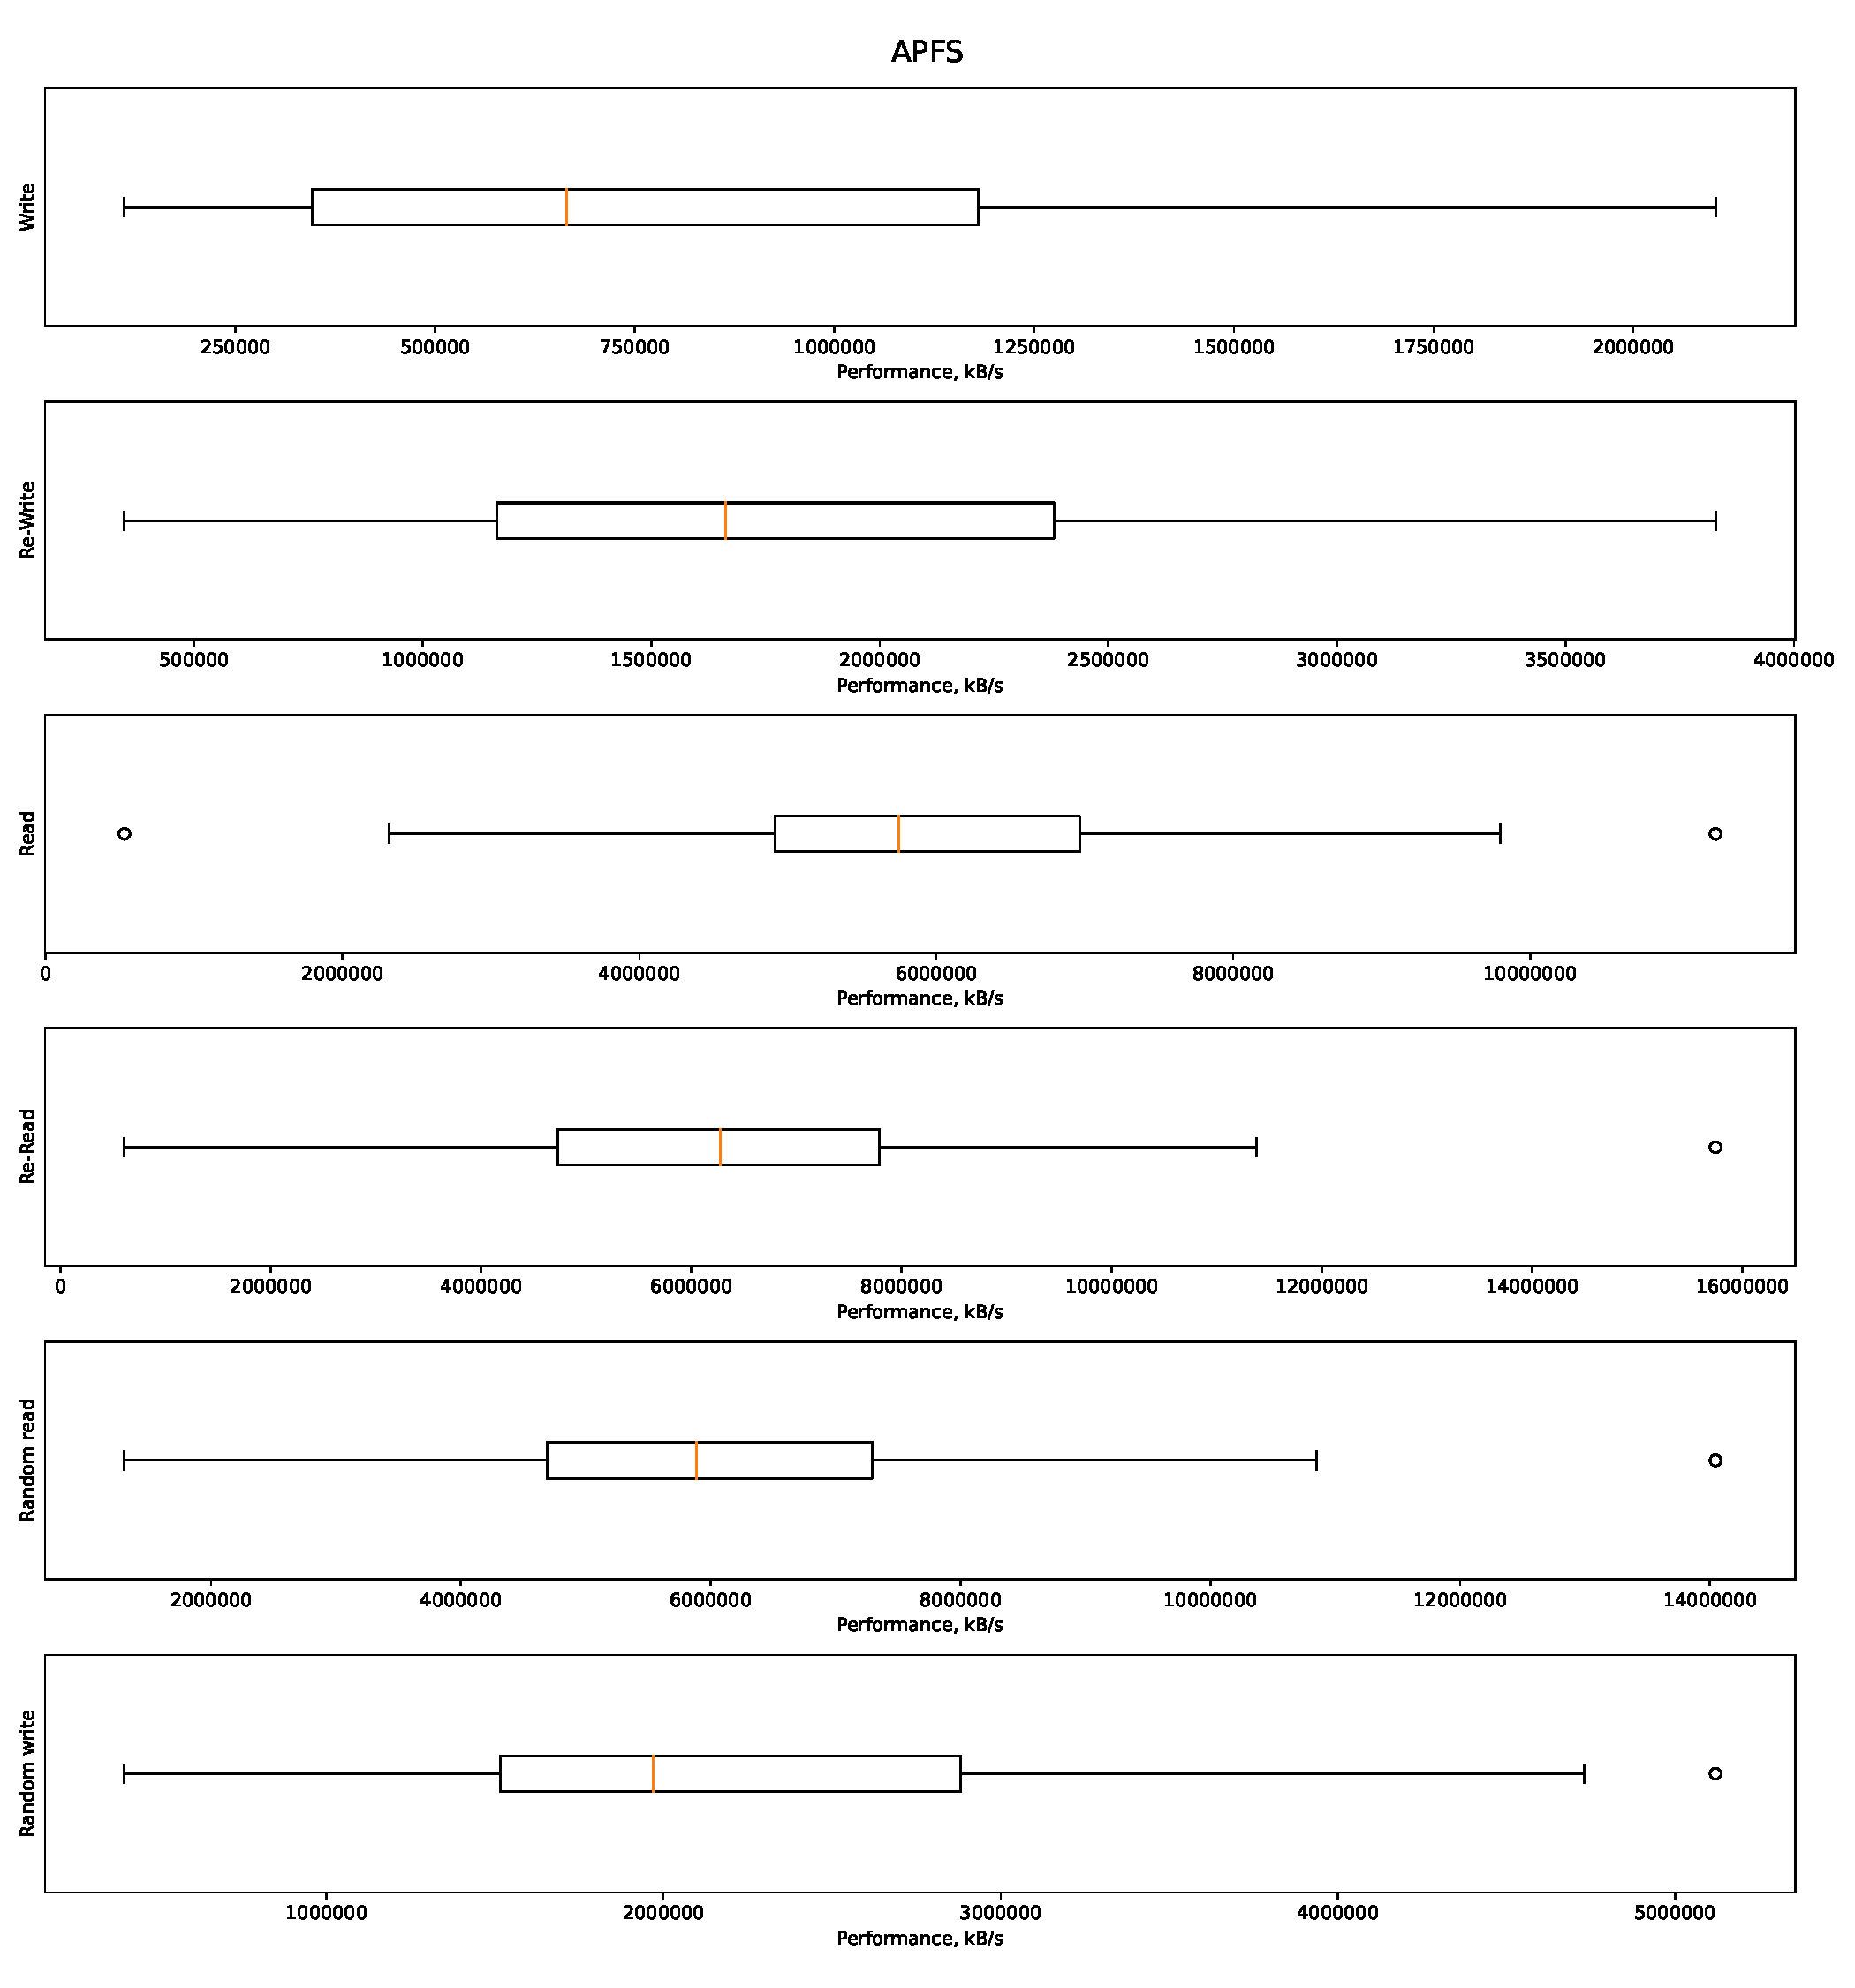
\includegraphics[width=1.0\textwidth]{figures/benchmarking/local/APFS-box.pdf}
	\end{center}
	\caption{Box plot of the IOZone output for the different tests for APFS}
\end{figure}

Comparing the Fejk FFS (FFFS) benchmarking results against the APFS benchmarking results, we can compare the theoretical best performance of FFS against a general-purpose highly-used filesystem. In Table~\ref{tbl:data_read_fejk_ffs} and Table~\ref{tbl:data_read_apfs} we can see that the read operation perform almost similarly for FFFS and APFS, where APFS is in general faster than FFFS. However, for certain data points, such as \texttt{file size = 4096kB, buffer size = 4kB}, FFFS has higher throughput than APFS with \SI[per-mode = symbol]{2\,866\,270}{\kilo\byte\per\second} for FFFS and \SI[per-mode = symbol]{2\,402\,508}{\kilo\byte\per\second} for APFS. The cache of the filesystems can influence the performance of the read operation a lot. In the case of FFFS, the filesystem will cache the written data as long as its size is less the limit of \SI{5}{\mega\byte}. However, there is no significant difference between the FFFS performance of reading a file that fits in the FFFS cache, and one that does not. All files that are read in FFFS that are not in the FFFS cache are read from disk, which invokes at least one APFS read operation. While the APFS read operation called might not be called with the same buffer size as the read operation called by IOZone on FFFS, the performance of the FFFS read operation cannot exceed the APFS read operation. However, the similarity of the performance between the filesystem indicates that FFS implements fast read operations, and that the read operation performance of FFS depends to a high extent on the internet bandwidth and latency to the OWS, as well as the OWS's data processing performance.

While the values of the read operation for FFFS and APFS are comparable to each other, this is not the case for all tests. For instance is the write operation of FFFS much slower than the write operation of APFS as can be seen in Table~\ref{tbl:data_write_fejk_ffs} and Table~\ref{tbl:data_write_apfs}. The write operation of FFFS has about 2-3\% the performance of the write operation of APFS. The reason for this can be the fact that FFFS has to encrypt the data stored, including creating all the cryptographic variables such as the salt and the IV. While APFS is also an encrypted filesystem, it is possible that the cryptographic functions are much faster than for FFFS as they for instance can be run in kernel space, while FFFS is running in user space.